% Chapter 

\chapter{Go-op} % Main chapter title
\label{Goop} % For referencing the chapter elsewhere, use \ref{Chapter1} 

This chapter introduces the Go-op application in it's current state of development.

%%%%%%%%%%%%%%%%%%%%%%%%%%%%%%%%%%%%%%%%%%%%%%%%%%%%
\section{Welcome Page}
\begin{figure}
\centering
\makebox[\textwidth][c]{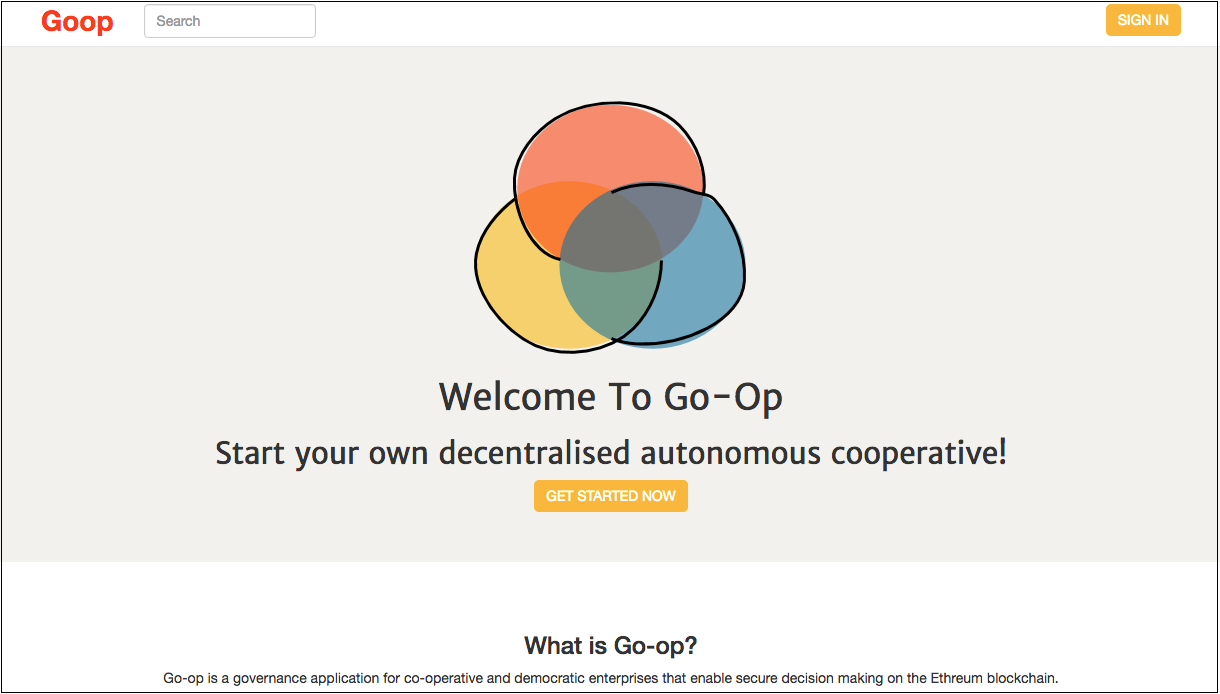
\includegraphics[width=1.4\textwidth]{Figures/WelcomePage}}
\decoRule
\caption[Go-op Welcome Page]{Landing page for Go-op application}
\label{fig:welpage}
\end{figure}

The landing or welcome page for Go-op is shown in figure \ref{fig:welpage}. This is the first page a user will see when they load the application. It's purpose is to attract the users attention and describe the premise of the Go-op. By clicking the orange buttons to 'sign up' or 'get started now', the user will be taken to the registration page.\\

%%%%%%%%%%%%%%%%%%%%%%%%%%%%%%%%%%%%%%%%%%%%%%%%%%%%
\section{Registration}
\begin{figure}
\centering
\makebox[\textwidth][c]{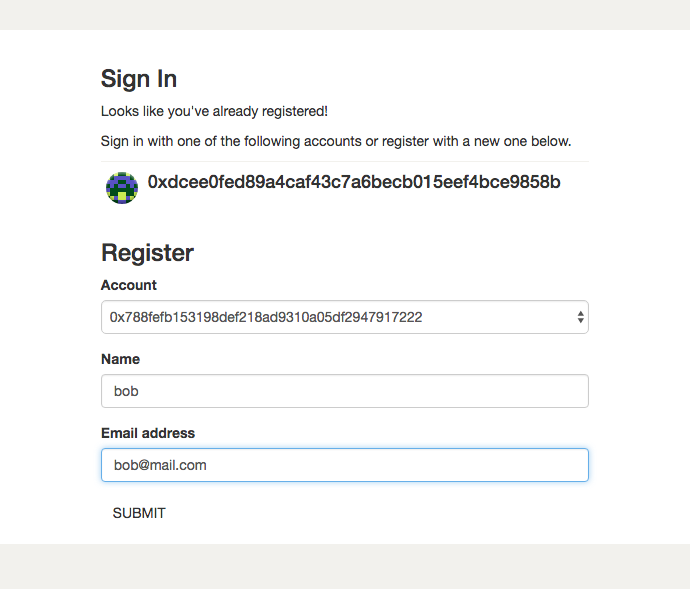
\includegraphics[width=1.4\textwidth]{Figures/RegistrationPage2}}
\decoRule
\caption[Go-op Registration View]{Go-op registration view.}
\label{fig:regpage}
\end{figure}

Users 'sign up' to Go-op through the registration page, figure \ref{fig:regpage}. The registration process associates a user's Ethereum account with their personal details. Ethereum accounts are managed by an external entity such as the local Ethereum client or by a Web3 browser such as Mist. Users are able to register an identity for each of their Ethereum accounts.\\

The only personal details currently required by Go-op are name and email address. Our research into membership application forms found that the information gathered by most coops is usually a name, address, telephone number and email. At this stage in development it is not yet clear whether a subset of this information will be sufficient for digital governance. It was decided that the PoC should be kept as simple as possible without introducing too many unvalidated features. 

% Future development work should proceed in tighter communication with cooperatives to vali

%%%%%%%%%%%%%%%%%%%%%%%%%%%%%%%%%%%%%%%%%%%%%%%%%%%%
\section{Home Page}

\begin{figure}
\centering
\makebox[\textwidth][c]{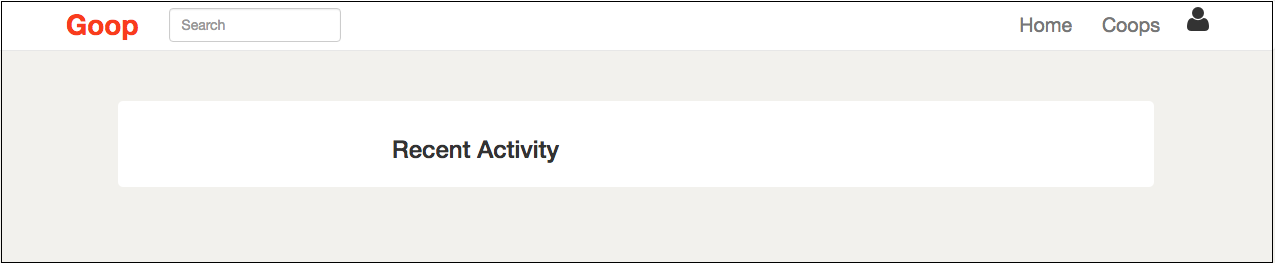
\includegraphics[width=1.4\textwidth]{Figures/HomePage}}
\decoRule
\caption[Go-op User Home Page View]{Go-op user home page view.}
\label{fig:homepage}
\end{figure}

The user 'home page', shown in figure \ref{fig:homepage}, currently has no functionality. In future, the homepage should act as a quick reference panel for a user to identify recent changes with their co-operatives. The information we hope to populate this page with are new membership events, new proposal creation events and new proposal conclusion events.\\
 
%%%%%%%%%%%%%%%%%%%%%%%%%%%%%%%%%%%%%%%%%%%%%%%%%%%%
\section{My Coops}

\begin{figure}
\centering
\makebox[\textwidth][c]{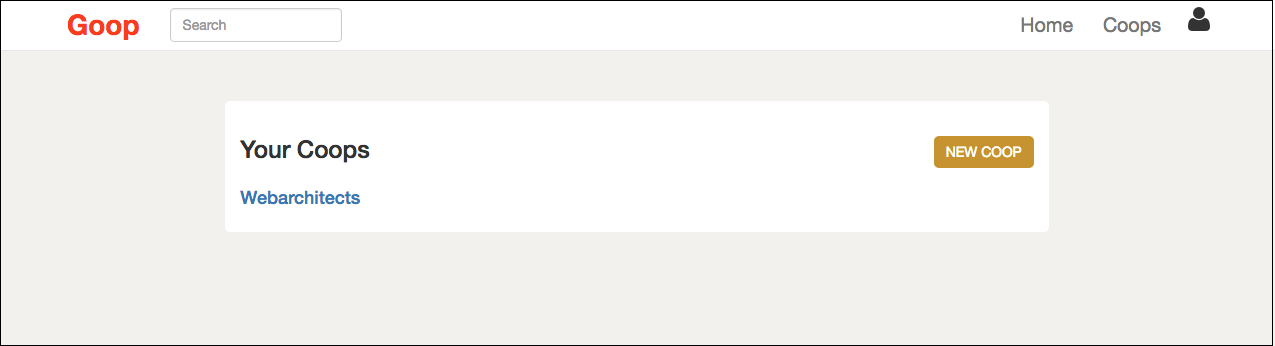
\includegraphics[width=1.4\textwidth]{Figures/MyCoopsPage}}
\decoRule
\caption[Go-op My Coops View]{Go-op my coops view.}
\label{fig:coopspage}
\end{figure}

The 'my coops' page, shown in figure \ref{fig:coopspage}, is a simple navigation page that displays all the co-operatives a user is a member of. Figure \ref{fig:coopspage} shows that the logged in user is a member of one co-operative called 'Webarchitects'. Users can set up a new co-operative on this page by clicking the 'new coop' button.\\

\subsection{Creating A Coop}

\begin{figure}
\centering
\makebox[\textwidth][c]{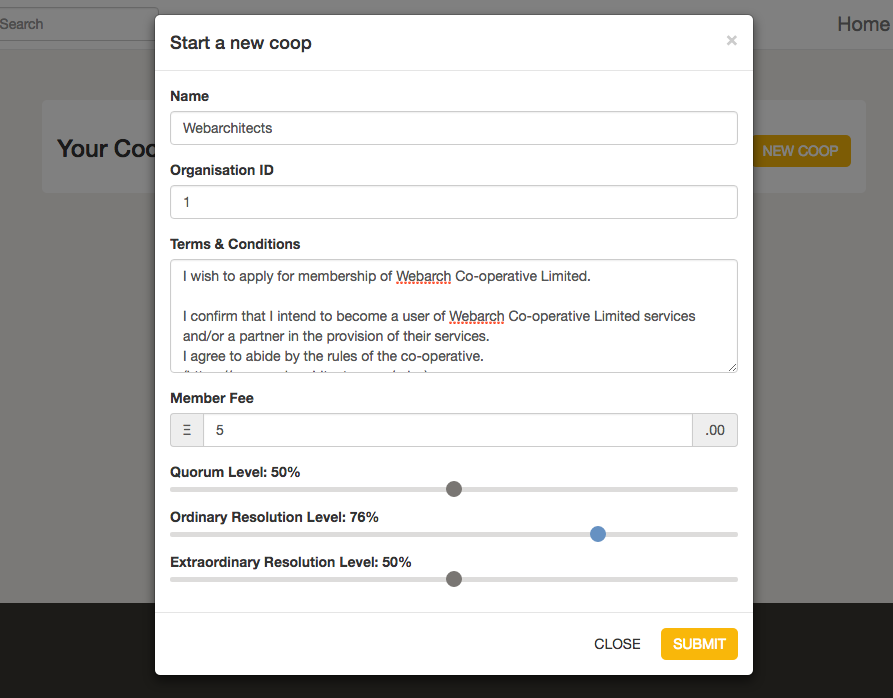
\includegraphics[width=1.4\textwidth]{Figures/CreateCoopPage}}
\decoRule
\caption[Go-op New Coop Pop Up]{Go-op coop creation pop up.}
\label{fig:createcooppage}
\end{figure}

Figure \ref{fig:createcooppage} shows the pop up modal for creating a new co-operative. To set up a new co-operative a user must provide a name, Coops UK ID, Terms \& Conditions (for membership), membership fee (in Ether), quorum level and resolution levels (see section \ref{subsec:CooperativeGovernance} for more information).\\

The terms and conditions and membership fee are made visible to users when they join a co-operative. The quorum and normal resolution levels are used by Go-op to determine whether ordinary proposals tabled by members of the co-operative are passed or defeated. The extraordinary resolution level is not currently used by Go-op. In future, Go-op could allow it's members to table a second type of proposal to change the 'rules' of the co-operative itself (such as changing the quorum level). The extraordinary resolution level would define the level of agreement required for these kinds of proposals to pass. \\

The Coops UK ID is also not currently used by Go-op. At the moment, anyone can set up a co-operative on Go-op but in future, assurances around 'co-operative identity' may become a requirement. Because all real co-operatives should already have a Coops UK ID, providing it during creation could allow Coops UK to easily validate co-operatives signing up to Go-op.\\
 

%%%%%%%%%%%%%%%%%%%%%%%%%%%%%%%%%%%%%%%%%%%%%%%%%%%%
\section{Coop Page}

\begin{figure}
\centering
\makebox[\textwidth][c]{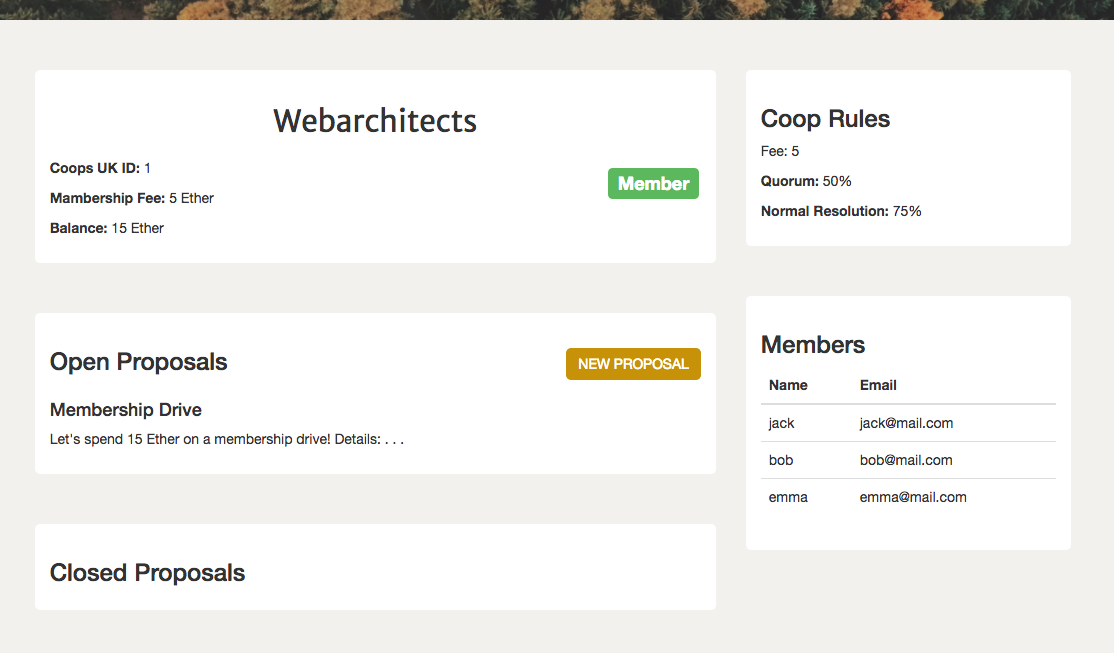
\includegraphics[width=1.4\textwidth]{Figures/CoopPage2}}
\decoRule
\caption[Go-op Coop Home Page]{Go-op coop home page.}
\label{fig:cooppage}
\end{figure}

Figure \ref{fig:cooppage} shows the home page for a co-operative. The page is split into five sections: title, rules, members, open proposals and closed proposals. The title section displays key information such as the name of the cooperative, it's balance (accumulated membership fees etc), it's membership fee and it's Coops UK ID. The 'rules' section lists the rules for quorum and resolution. The 'members' section is simply a list of members. The open proposals allows users to view proposals for which voting is still open and allows users to table new proposals. The closed proposals serves as an audit for closed and decided proposals. \\

\subsection{Creating A Proposal}

\begin{figure}
\centering
\makebox[\textwidth][c]{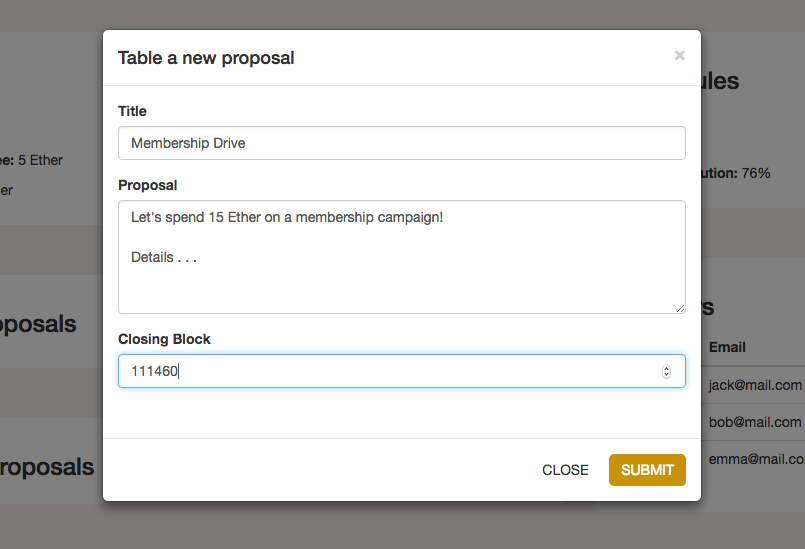
\includegraphics[width=1.4\textwidth]{Figures/NewProposalPage}}
\decoRule
\caption[Go-op New Proposal Pop Up]{Go-op new proposal pop up.}
\label{fig:createproposal}
\end{figure}

Clicking on the 'new proposal' button in the 'open proposals' section opens the 'new proposal' dialog shown in figure \ref{fig:createproposal}. This is a simple form with three fields: title, proposal text and closing block. The closing block determines the block on which the vote is scheduled to close. Because Go-op uses the Ethereum Alarm Clock as the underlying scheduling system (see section\ref{sec:blocktime}), a block number is the most precise way a closing date can be specified. This is reasonably ugly feature that pierces the abstraction of blockchain technology from end users. Ideally, users should specify closing dates in terms of time. This may be possible if Go-op switches to a lazy evaluation approach as discussed in section \ref{sec:blocktime}. At the very least, the form should provide extra information about the estimated processing dates for any block in the future. 
 

\subsection{Voting On A Proposal}
\begin{figure}
\centering
\makebox[\textwidth][c]{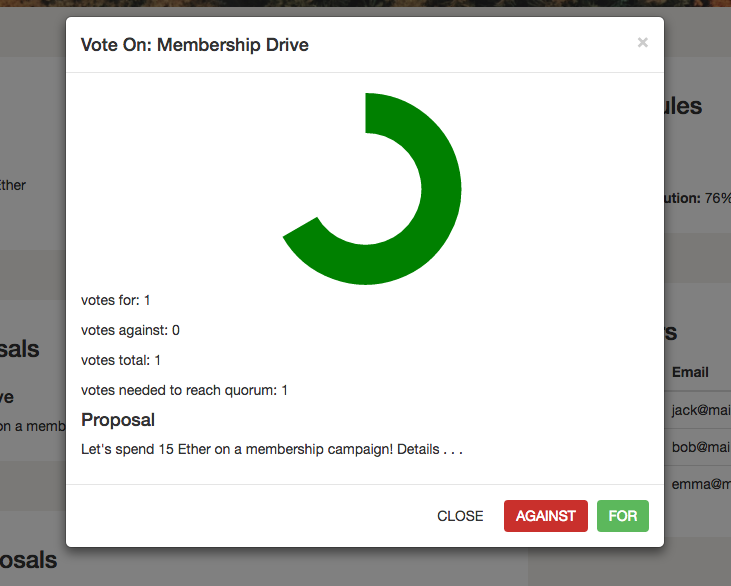
\includegraphics[width=1.4\textwidth]{Figures/ProposalVotePage}}
\decoRule
\caption[Go-op Proposal Pop Up]{Go-op proposal pop up.}
\label{fig:proposalvote}
\end{figure}

Figure \ref{fig:proposalvote} shows the pop up for an open proposal. The pop up includes information on the actual proposal as well as the number of votes for, votes against, total votes and number of votes required to reach quorum. This information is also summarised graphically in a simple 'doughnut' chart. The empty space in the doughnut chart illustrates the percentage of votes still required to reach quorum. There are three buttons at the foot of the pop up which allow a user either close the pop up or vote for or against the proposal.\\

When a proposal closes it becomes listed in the 'closed proposals' section of the coop home page. Pop ups for closed proposals look identical as for open proposals except that there are no buttons for voting.\\

\section{Loading Screens}
\begin{figure}
\centering
\makebox[\textwidth][c]{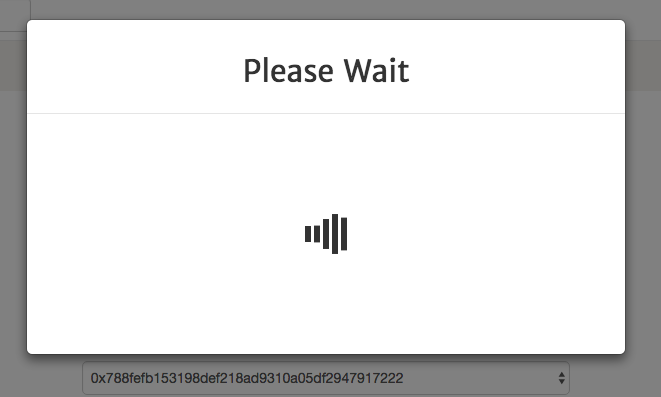
\includegraphics[width=1.4\textwidth]{Figures/WaitPage}}
\decoRule
\caption[Go-op Loading Pop Up]{Go-op loading pop up.}
\label{fig:waitpage}
\end{figure}

Many user interactions spawn transactions that need to be mined into the blockchain. Loading modals, such as the one shown in figure \ref{fig:waitpage}, are used to avoid unresponsive views while the application waits for transactions to be processed. Whilst this is nice, transactions can take up to thirty seconds to get mined which is a long time to look at a loading screen. A better solution for the future would be an optimistic UI that simply assumes transactions will be successful when it can be confident. Some kind of icon could be used to show which aspects of the UI have been confirmed in the blockchain and which components are still pending.
















